\section{Software Licenses}\label{licenses}

\begin{flushleft}
	Every business uses software to manage business processes, communicate with
	employees, customers, and vendors, and for myriad other purposes. In most instances,
	software products require activating licenses or agreeing to ``terms and conditions''
	before programs can be downloaded, installed, or accessed. There are many types
	of software licenses, with different terms, support agreements, restrictions, and
	costs. Users need to understand the basics of software licenses, to ensure a
	full understanding of responsibilities and compliance with legal terms and
	limitations.
\end{flushleft}

\begin{flushleft}
	A software license is a contract between the entity that created and supplied
	an application, underlying source code, or related product and its end user.
	The license is a text document designed to protect the intellectual property
	of the software developer and to limit any claims against them that may arise
	from its use. A software license also provides legally binding definitions for
	the distribution and use of the software. End-user rights, such as installation,
	warranties, and liabilities, are also often spelled out in the software license,
	including protection of the developer's intellectual property.
\end{flushleft}

\subsection{Types of Licenses}\label{license-types}

\begin{flushleft}
	\textbf{Public Domain:} This is the most permissive type of software license.
	When software is in the public domain, anyone can modify and use the software
	without any restrictions. But you should always make sure it's secure before
	adding it to your own codebase. Warning: Code that doesn't have an explicit
	license is NOT automatically in the public domain. This includes code snippets
	you find on the internet.
\end{flushleft}

\begin{flushleft}
	\textbf{Permissive:} Permissive licenses are also known as ``Apache style'' or
	``BSD style.'' They contain minimal requirements about how the software can be
	modified or redistributed. This type of software license is perhaps the most
	popular license used with free and open source software. Aside from the Apache
	License and the BSD License, another common variant is the MIT License.
\end{flushleft}

\begin{flushleft}
	\textbf{LGPL:} The GNU Lesser General Public License allows you to link to open
	source libraries in your software. If you simply compile or link an LGPL-licensed
	library with your own code, you can release your application under any license
	you want, even a proprietary license. But if you modify the library or copy
	parts of it into your code, you'll have to release your application under similar
	terms as the LGPL.
\end{flushleft}

\begin{flushleft}
	\textbf{Copyleft:} Copyleft licenses are also known as reciprocal licenses or
	restrictive licenses. The most well-known example of a copyleft or reciprocal
	license is the GPL. These licenses allow you to modify the licensed code and
	distribute new works based on it, as long as you distribute any new works or
	adaptations under the same software license. For example, a component's license
	might say the work is free to use and distribute for personal use only. So any
	derivative you create would also be limited to personal use only. (A derivative
	is any new software you develop that contains the component.) The catch here is
	that the users of your software would also have the right to modify the code.
	Therefore, you'd have to make your own source code available. But of course,
	exposing your source code may not be in your best interests.
\end{flushleft}

\begin{flushleft}
	\textbf{Propriety:} Of all types of software licenses, this is the most restrictive.
	The idea behind it is that all rights are reserved. It's generally used for
	proprietary software where the work may not be modified or redistributed.
\end{flushleft}

\subsection{Legal Terms}\label{license-legal-terms}

\begin{itemize}
	\item \textbf{Commercial Use:} Describes the ability to use the software for commercial purposes.
	\item \textbf{Modify:} Describes the ability to modify the software and create derivatives.
	\item \textbf{Distribute:} Describes the ability to distribute original or modified (derivative) works.
	\item \textbf{Place Warranty:} Describes the ability to place warranty on the software licensed.
	\item \textbf{Sublicense:} The LGPL prohibits sublicensing, yet each user that receives the software automatically has the right to run, modify and distribute the work.
	\item \textbf{Use Trademark:} You may not use the names of the original company or its members to endorse derived products.
	\item \textbf{Hold Liable:} Describes the warranty and if the software/license owner can be charged for damages.
	\item \textbf{State Changes:} Stating significant changes made to software.
	\item \textbf{Disclose Source:} If you distribute this library in an executable, you must make the source available for 3 years.
	\item \textbf{Include Original:} Describes whether copies of the original software or instructions to obtain copies must be distributed with the software.
	\item \textbf{Include Copyright:} Describes whether the original copyright must be retained.
	\item \textbf{Include License:} Including the full text of license in source or object code copies.
	\item \textbf{Include Install Instructions:} If the software is part of a consumer device, you must include the installation information necessary to modify and reinstall the software.
	\item \textbf{Include Note:} If the library has a "NOTICE" file with attribution notes, you must include that NOTICE when you distribute. You may append to this NOTICE file.
\end{itemize}

\subsection{Copyleft vs Copyright}\label{copyleft-vs-copyright}

\begin{flushleft}
	A copyright is a legal right bestowed upon creators of original works to dictate
	how those works can or cannot be copied, modified, and distributed by others. If
	someone uses or distributes an original work in a way that's contrary to what its
	creator allows (``infringement''), the creator is entitled to seek legal action.
\end{flushleft}

\begin{flushleft}
	Copyleft is a term coined by Richard Stallman who originally used this term to
	distinguish his way of free software licensing (such as GPLv3 or LGPLv3) from
	the other Copyright licenses which are typically designed by proprietary companies
	to keep the holding rights of a software to themselves by not disclosing the source
	code. The Free Software Foundation (FSF) is a  is a nonprofit organization that set
	out to promote the usage and development of free software\footnote{\href{https://www.gnu.org/philosophy/free-sw.html.en}{What is Free Software?}}.
\end{flushleft}

\begin{flushleft}
	It's important to point out that the term copyleft holds no legal significance
	in any court of the world because it was never really defined under the law.
	However, the terms and conditions of copyleft licenses such as GPLv3 are legally
	binding. On a related note, the terms Share-Alike and Copyleft are for the most
	part synonymous, with the exception that Share-Alike licenses are fit for use for
	works of art, while copyleft licenses were designed with software development in
	mind. The main idea behind copyright is that creators restrict what others can or
	cannot do with their works and must grant individual permission to do otherwise.
	Copyleft licenses exist within the legal structure of copyrights and grants the
	user permission to copy, modify and distribute works in any fashion they like.
	Failing to abide to the rules that are governed by copyleft licenses provides
	the project maintainer with legal grounds for action. While copyleft licenses are
	very permissive with regards to the users freedom, it also imposes a series of
	demands that are to be kept up by the developers, which most notably includes
	the requirement that any derivative works must be published under a license that
	grants the same rights as the license of the pulled-in dependency.
\end{flushleft}

\subsection{Common Licenses}\label{common-licenses}

\subsubsection{MIT}

\begin{flushleft}
	If you use the MIT license, you \emph{can} do any of the following:
\end{flushleft}

\begin{enumerate}
	\item Commercial Use
	\item Modify
	\item Sublicense
	\item Private Use
\end{enumerate}

\begin{flushleft}
	If you use the MIT license, you \emph{canont} do any of the following:
\end{flushleft}

\begin{enumerate}
	\item Hold Liable
\end{enumerate}

\begin{flushleft}
	If you use the MIT license, you \emph{must} do all of the following:
\end{flushleft}

\begin{enumerate}
	\item Include Copyright
	\item Include License
\end{enumerate}

% ===

\subsubsection{GPLv3}

\begin{flushleft}
	If you use the GPLv3 license, you \emph{can} do any of the following:
\end{flushleft}

\begin{enumerate}
	\item Commercial Use
	\item Modify
	\item Distribute
	\item Place Warranty
	\item Use Patent Claims
\end{enumerate}

\begin{flushleft}
	If you use the GPLv3 license, you \emph{canont} do any of the following:
\end{flushleft}

\begin{enumerate}
	\item Sublicense
	\item Hold Liable
\end{enumerate}

\begin{flushleft}
	If you use the GPLv3 license, you \emph{must} do all of the following:
\end{flushleft}

\begin{enumerate}
	\item Include Original
	\item State Changes
	\item Disclose Source
	\item Include Copyright
	\item Include License
	\item Include Install Instructions
\end{enumerate}

% ===

\subsubsection{LGPLv3}

\begin{flushleft}
	If you use the LGPLv3 license, you \emph{can} do any of the following:
\end{flushleft}

\begin{enumerate}
	\item Commercial Use
	\item Modify
	\item Distribute
	\item Place Warranty
	\item Use Patent Claims
\end{enumerate}

\begin{flushleft}
	If you use the LGPLv3 license, you \emph{canont} do any of the following:
\end{flushleft}

\begin{enumerate}
	\item Sublicense
	\item Hold Liable
\end{enumerate}

\begin{flushleft}
	If you use the LGPLv3 license, you \emph{must} do all of the following:
\end{flushleft}

\begin{enumerate}
	\item Include Original
	\item State Changes
	\item Disclose Source
	\item Include Copyright
	\item Include License
	\item Include Install Instructions
\end{enumerate}

% ===

\subsubsection{Apache License 2.0}

\begin{flushleft}
	If you use the Apache License 2.0, you \emph{can} do any of the following:
\end{flushleft}

\begin{enumerate}
	\item Commercial Use
	\item Modify
	\item Distribute
	\item Sublicense
	\item Private Use
	\item Place Warranty
\end{enumerate}

\begin{flushleft}
	If you use the Apache License 2.0, you \emph{canont} do any of the following:
\end{flushleft}

\begin{enumerate}
	\item Hold Liable
	\item Use Trademark
\end{enumerate}

\begin{flushleft}
	If you use the Apache License 2.0, you \emph{must} do all of the following:
\end{flushleft}

\begin{enumerate}
	\item Include Copyright
	\item Include License
	\item State Changes
	\item Include Notice
\end{enumerate}

% ===

\subsubsection{BSD-3 Clause (Revised)}

\begin{flushleft}
	If you use the BSD-3 Clause (Revised) license, you \emph{can} do any of the following:
\end{flushleft}

\begin{enumerate}
	\item Commercial Use
	\item Modify
	\item Distribute
	\item Place Warranty
\end{enumerate}

\begin{flushleft}
	If you use the BSD-3 Clause (Revised) license, you \emph{canont} do any of the following:
\end{flushleft}

\begin{enumerate}
	\item Use Trademark
	\item Hold Liable
\end{enumerate}

\begin{flushleft}
	If you use the BSD-3 Clause (Revised), you \emph{must} do all of the following:
\end{flushleft}

\begin{enumerate}
	\item Include Copyright
	\item Include License
\end{enumerate}

\subsection{License Compatibility}

\begin{flushleft}
	Before you can determine which licenses govern any reused code in your codebase,
	you need to create a software bill of materials, or a list of all the components
	in your code. And the fastest way to generate that list is with a software composition
	analysis tool. A good SCA tool will be able to find full components as well as
	code snippets, and it'll tell you which licenses apply to each piece of code and
	whether you might be using licenses that have conflicts.
\end{flushleft}

\begin{flushleft}
	The licences for distributing free or open source software (FOSS) are divided
	in two families: permissive and reciprocal (or ``copyleft''). Permissive licenses
	(BSD, MIT, X11, Apache, Zope) are generally compatible and interoperable with most
	other licences, tolerating to merge, combine or improve the covered code and to
	re-distribute it under many licences (including non-free or ``proprietary'').
\end{flushleft}

\begin{flushleft}
	At the contrary, the reciprocal licences impose to provide back the source code
	under the same license in case of distribution, when the distributed work is
	a derivative of the covered work. To avoid software appropriation by third
	parties, many open source projects have adopted reciprocal licensing terms:
	this is the case of the two Gnu GPLs and the EUPL.
\end{flushleft}

\begin{flushleft}
	Some licences like the LGPL or the MPL try to compromise between the permissive
	and reciprocal requirements: covered components (and their specific derivatives)
	will always keep their primary license, but the combined application ``as a whole''
	(even if it may be considered globally as a derivative) or its executable binary
	(a single program from the user point of view) can be distributed under any license.
\end{flushleft}

\begin{flushleft}
	In most cases, permissive licenses are also compatible with copyleft licenses.
	There are two exceptions to this rule: The Apache 2.0 license and the original
	(4-clause) BSD license. The Apache 2.0's license partner rights make it incompatible
	with GPLv2, but it is compatible with GPLv3. The 4-clause BSD license's advertising
	clause makes it incompatible with all copyleft licenses. The modified (3-clause)
	BSD license doesn't include the problematic advertising clause, so it is compatible.
\end{flushleft}

\begin{flushleft}
	The most problematic practice is combining two copyleft licenses. As a rule of
	thumb, copyleft licenses are incompatible unless they have explicit compatibility
	provisions. As Richard Stallman, creator of the GNU GPL license:
\end{flushleft}

\begin{displaycquote}
	``If license A says extended programs must be under license A, and license B
	says extended programs must be under license B, they have an irreconcilable
	disagreement; the license of the combined program would have to be A, and it
	would have to be B.''
\end{displaycquote}

\begin{flushleft}
	\textbf{Compatibility} is the possibility to combine or merge software code
	covered by several licences and to distribute the combined work. At the contrary,
	license incompatibility exists when a program is derivative of components licensed
	under two different reciprocal licences (for example, the GPLv2, which is still
	the most used copyleft licence, is not compatible with GPLv3, and vice-versa).
\end{flushleft}

\begin{flushleft}
	\textbf{Interoperability} is another legal concept originally defined by Directive
	91/250/EEC as "the ability to exchange information and mutually to use the
	information which has been exchanged" (Recital 10). And to implement interoperability,
	the reproduction of ``interfaces'' (also defined in as ``the parts of the program
	which provide for interconnection and interaction between elements of software'') is
	authorized as a copyright exception to the author's exclusive rights (possibly
	formalized in a copyright license), This is the reason why the EUPL, by application
	of EU law, is interoperable. This is a major difference with some other reciprocal
	licences (mainly the GPLv2, GPLv3 and AGPL) where the license steward states that
	static or dynamic linking extend their copyright.
\end{flushleft}

\begin{flushleft}
	A logical incompatibility issue may be resolved through \textbf{Dual Licensing}: the
	original licensor (owning full copyright) may provide the same program under two or
	more licences, even if these licenses are not compatible. The most frequent cases
	apply to licensors distributing their work under the ``GPL'' (without mentioning
	the version number, or adding "or later"): in such case, recipients can use the
	work under any of these licences (GPLv2 or GPLv3), which is in practice a dual
	licensing. When the licences are mutually incompatible, the risk of dual licensing
	is the forking of the program in various legally incompatible releases, which even
	the original licensor will not be able to reunify.
\end{flushleft}

\begin{figure}[ht]
	\centering
	% https://i.imgur.com/ejucFRV.png
	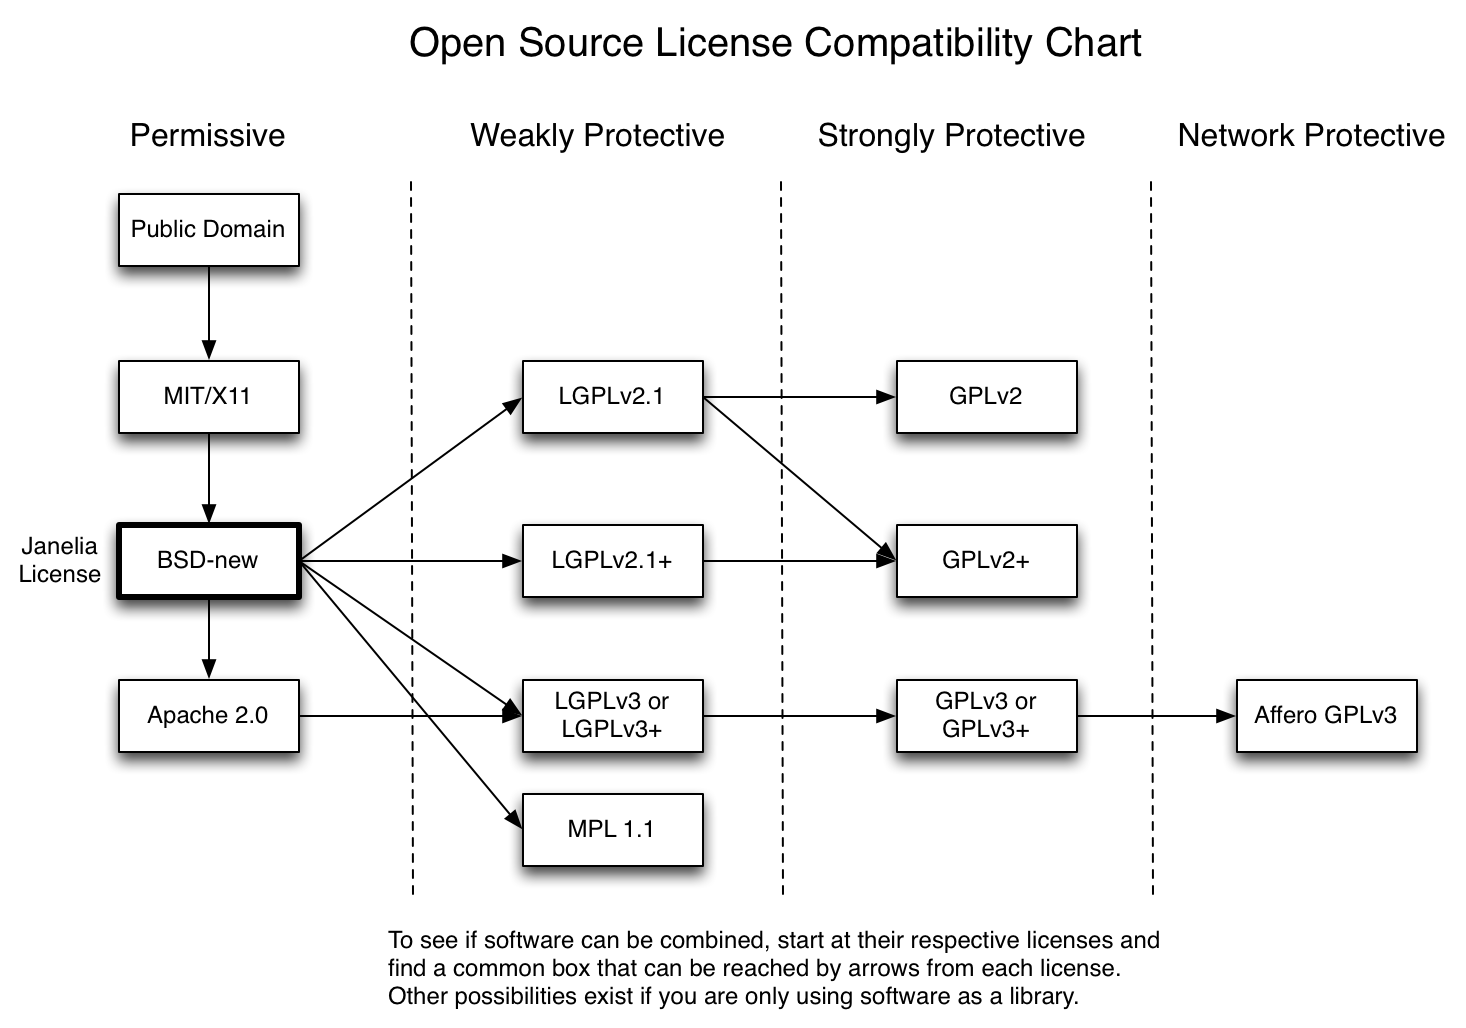
\includegraphics[scale=0.4]{images/open_licenses.png}
	\caption{FOSS License Compatibility}\label{fig:foss-licenses}
\end{figure}

\begin{flushleft}
	In this figure, the boxes are the names of different FLOSS licenses. An arrow
	from box A to box B means that you can combine software with these licenses;
	the combined result effectively has the license of B, possibly with additions
	from A. To see if software can be combined, start at their respective
	licenses, and find a common box by following the arrows. For example, Apache 2.0-licensed
	software and GPLv2+-licensed software can both reach "GPLv3 or GPLv3+", so they
	can be combined using GPLv3 or GPLv3+.
\end{flushleft}
